\documentclass{article}
\usepackage{graphicx}
\usepackage{fancyhdr}
\usepackage{wrapfig}
\usepackage[margin=1.5in]{geometry}
% Introduction and background (1 page)
% Literature review (1/2 page)
% Dataset Description and exploratory data analysis of the dataset (1-2 page)
% Proposed methodology (1 page)
% Experimental results (2-3 pages)
% Conclusion and discussion -- you can include the project roadmap here too (1/2 page)
% References (no limit)
\linespread{1}
\pagestyle{fancy}
\title{\textbf{Credit Score Classification}}
\author{Kyle Jow, Jimmy Nguyen, Kyle Pickle, Jacob Tuttle, Kris Wong}
\date{December 2023}

\begin{document}
\pagenumbering{gobble}
\maketitle
\newpage
\pagenumbering{arabic}
\pagestyle{fancy}
\fancyhf{} % clear header and footer
\fancyhead[R]{Credit Score Classification}
\fancyfoot[R]{\thepage}
\section*{Introduction and background}
A common problem in the finance and banking industry is assessing the risk involved with lending money to a client.
To better assess a borrower's creditworthiness, lenders formulate and assign “credit scores” to their clients, based on preconceived data 
like income, spending, and credit history.
This score can then be used by a bank as an indicator of whether a client will default or otherwise miss a payment on a given loan.
The rise of cloud-based computing in the 21st century has made it more advantageous and easier than ever for banks to seamlessly share a
standardized database of credit scores and financial information their clients.
As a result, credit scoring is being used more and more frequently to determine your “worthiness” for almost anything -- qualifying for
mortgages, insurance, even less common things like cell phone plans and even your employability.
\vspace{5mm}\newline
With this increase in credit scoring came an increased interest in financial literacy among clients and how to understand and improve their
scores.
As such, credit standards like FICO and VantageScore have begun giving their clients a way to view an estimation of their credit score, often
provided through the bank and credit card services that utilize them.
These credit score estimates are predicted in a way that is simple for the client to understand, often broken down into categories like
“poor,” “standard,” and “good” and given alongside graphs displaying factors like age bracket and income to put them into perspective.
This demand for straightforward and transparent credit scoring has compelled banks to consider less intricate or “black box” machine
learning models, leading to a delicate balance between accuracy and simplicity.
\vspace{5mm}\newline
Credit scoring is considered to be one of first and most common instances of machine learning used in the field of economics.
The financial sector is always historically one of the first sectors to adopt technological advancements like machine learning and AI,
and with so much data now digitized by banks alongside numerous complex variables that drive one's credit score, it has become a token
example of machine learning and how it allows us to not only predict creditworthiness but constantly tune the equations and hyperparameters
used to determine it in a fluctuating real-world economy.

% \newpage
\section*{Literature review}
One of the first fields machine learning techniques were tested in was economics,
particularly credit scoring. Researchers have utilized a variety of machine learning
algorithms to predict credit scores and risk. Common machine learning algorithms
used include logistic regression, support vector machines (SVM), and decision trees.
This section contains relevant work by researchers.
\vspace{5mm}\newline
% https://www.sciencedirect.com/science/article/pii/S0377221721005695#sec0012
Dumitrescu et. al. used a particular model for credit score classification with an 
improved logistic regression model that has non-linear decision tree effects. They created 
the penalised logistic tree regression, which predicted credit score 
more accurately than the benchmark logistic model commonly used in industry. The
datasets they used to test the robustness of the model --------
Additionally, they argue that this model preserves the interpretability of 
logistic regression, an aspect that makes logistic regression popular in industry. 
% https://www.spglobal.com/marketintelligence/en/news-insights/blog/machine-learning-and-credit-risk-modelling
Lei et.al. compare the performance of various models for predicting the probability 
of default. 

\newpage
\section*{Dataset description and exploratory data analysis}
The dataset contains 27 features. The features we will be focusing on in order
to classify a person's credit score, which is categorical, into either ``good", ``standard", or ``poor" credit
will be features that had the most correlation with credit score according to the heat map
generated from this data and features used in real-life credit score assessing. Although the Credit\_Utilization\_Ratio has little 
correlation to credit score, this feature is used to assess credit in real life, so we kept it. (Figure 1).\\
\begin{figure}[h]
    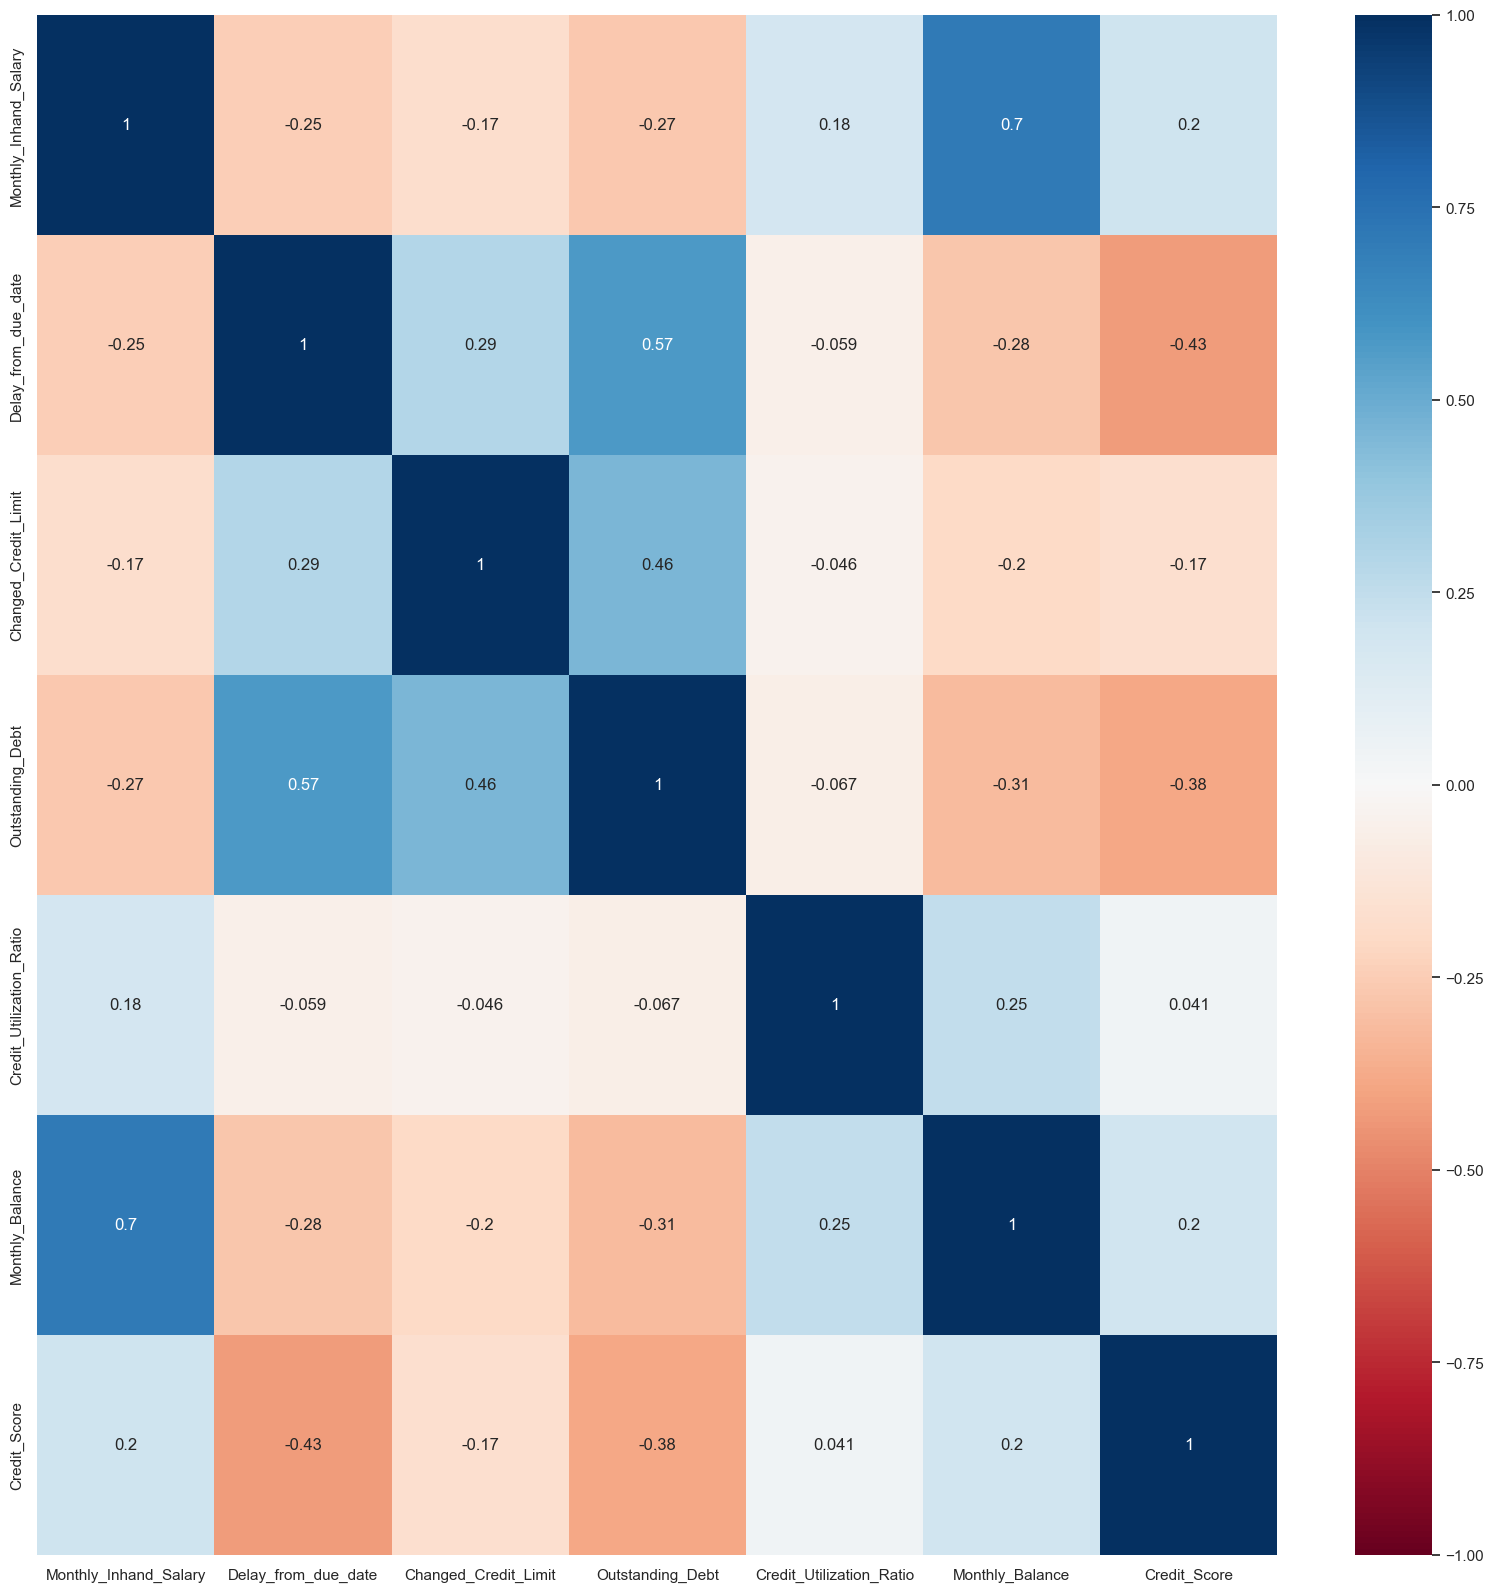
\includegraphics[width=\textwidth]{credscoreheatmap.png}
    \caption{Heat map correlation.}
    \label{fig:figure1}
\end{figure}
\newpage
\section*{Proposed methodology}
From the literature review and the fact that this problem involves multiclassification,
we decided to make and compare one SVM model and one multinomial logistic regression
model. Additionally, we used Streamlit to host our model online.

\section*{Experimental results}

\newpage
\section*{Conclusion and discussion}

\newpage
\section*{References}
\textbf{Dataset}\\
https://www.kaggle.com/datasets/parisrohan/credit-score-classification/data
\vspace{5mm}\newline
\textbf{Literature Review}\\
% https://www.sciencedirect.com/science/article/abs/pii/S0377221721005695
Dumitrescu, E., Hué, S., Hurlin, C., \& Tokpavi, S. (2022). 
Machine learning for credit scoring: Improving logistic regression 
with non-linear decision-tree effects. European Journal of Operational 
Research, 297(3), 1178-1192. doi:10.1016/j.ejor.2021.06.053
\vspace{5mm}\newline
%   talks about a modified logistic regression called "penalised 
%   logistic tree regression" that combines elements of decision trees and
%   logistic reg based on the adaptive lasso logistic regression model
% https://link.springer.com/chapter/10.1007/978-3-030-66891-4_5
% Guidolin, M., Pedio, M. (2021). Sharpening the Accuracy of Credit Scoring 
% Models with Machine Learning Algorithms. In: Consoli, S., Reforgiato Recupero, 
% D., Saisana, M. (eds) Data Science for Economics and Finance. Springer, Cham.
% https://doi.org/10.1007/978-3-030-66891-4\_5
% https://sci-hub.se/10.1057/jors.2009.129
% https://www.spglobal.com/marketintelligence/en/news-insights/blog/machine-learning-and-credit-risk-modelling
Yue, Lei, and Luka Vidovic. “Machine Learning and Credit Risk Modelling.”
 \textit{Machine Learning and Credit Risk Modelling $\vert$ S\&P Global Market Intelligence}, 
 S\&P Global Market Intelligence, 30 Nov. 2020, 
 www.spglobal.com/marketintelligence/en/news-insights/blog/machine-learning
 -and-credit-risk-modelling. 
\end{document}


% some drafts:
% https://sci-hub.se/10.1057/jors.2009.129
% interesting paper on showing weaknesses of evaluation statistics. not sure if its
% all that relevant though
% Hand and Zhou observe the performances of nine supervised learning 
% classification models in classifying customers in retail banking and discuss how 
% different commonly used methods such as area under curve (AUC), Gini measures, Kolmogorov–Smirnov statistic (KS), 
% used in  evaluating performance may give misleading conclusions due to 
% fundamental weaknesses behind these methods. For example, the KS statistic concluded that classification 
% trees performed the best while AUC ranks the model near the bottom.\\